\section{Preliminary models}
\label{Section:PreliminaryModels}
\subsection{Daimler models}
\label{Section:DaimlerModels}


%\subsubsection{Introduction}

Daimler use-case is based on two application scenarios \cite{Fer14}: i) early recognition of a lane change manoeuvre; and ii) earlier prediction of the need for a lane change based on relative dynamics between two vehicles driving in the same lane at different speeds. 

The first scenario has been previously addressed by Daimler \cite{kasper2012object}. The main result of this previous work was a static object-oriented Bayesian network (OOBN) \cite{KollerPfeffer1997} able to detect a manoeuvre 0.6 seconds before execution. The goal now is to enhance the prediction horizon for manoeuvre recognition by at least 1-2 seconds before execution to further improve the quality of the on-board adaptive cruise control. As we will explain later, this improvement is expected to be achieved by introducing a dynamic extension of the previously proposed static OOBN model. We basically consider such a dynamic extension for two main reasons: First, although with a limit prediction horizon, the static OOBN model has proven to be very robust for this task and it is considered as the gold-standard solution in Daimler. Second, the developed models in AMIDST project are expected to be integrated in an electronic control unit (ECU) \cite{Fer14}, so that the advances already made for the static model \cite{Weidl2014} could be exploited during the integration in the ECU of their dynamic counterparts. 

\subsubsection{Early recognition of a lane change manoeuvre}
\label{Section:Daimler:EarlyRecognition}

The basic settings of this application scenario are as follows: Let us suppose we are driving our car, referred to as EGO vehicle, in a highway. EGO vehicle is equipped with a video camera, radar, and some on-board sensors. Using the data provided by these sensors, the challenge consists in making an early recognition of a manoeuvre either by the EGO or any other relevant car in the traffic scene referred to as Object vehicle (OBJ). In total, the system is expected to recognise the following set of manoeuvres (a visual description of them is given below in Figure \ref{Figure:DaimlerManeuvers}):

\begin{enumerate}
\item \textbf{OBJ-CutIn}: A vehicle is moving to the lane where the EGO vehicle is placed.
\item \textbf{OBJ-CutOut}:  A vehicle that was driving in front of the EGO is leaving the EGO's lane.
\item \textbf{OBJ-Follow}: There is no lane change. The EGO is driving and there is another vehicle in front.
\item \textbf{LANE-Follow}: There is no lane change. The EGO is driving and there is no other vehicle in front.
\item \textbf{EGO-CutIn}: The EGO vehicle is moving right-direction to a new lane already occupied by another vehicle. 
\item \textbf{EGO-CutOut}: The EGO vehicle is leaving left-direction the lane where it was driving.
\end{enumerate}

\begin{figure}
\begin{center}
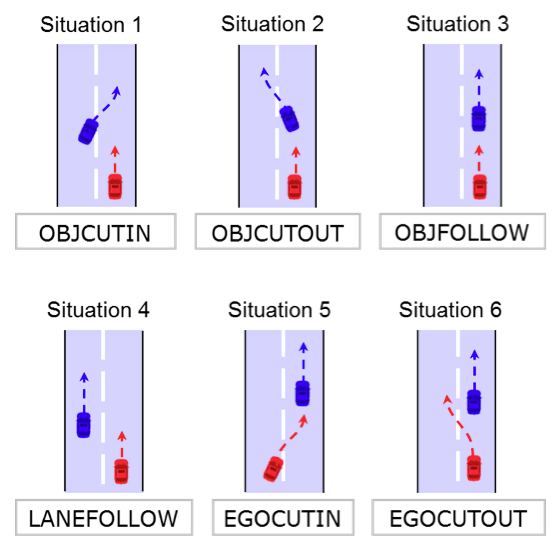
\includegraphics[scale=0.4]{./figures/DaimlerManeuvers}
\caption{\label{Figure:DaimlerManeuvers}The different manoeuvres to be identified by the AMIDST system. Red blocks represent the EGO vehicle while blue ones represent the Objet vehicle.}
\end{center}
\end{figure}

Instead of working directly with the raw data from the video, radar, and on-board sensors, the current manoeuvre recognition system uses the so-called ``object data'', which contains ``high level'' representations or features describing the traffic scene such as EGO's speed, distance between EGO and another vehicle in front, etc.  

\begin{figure}
\begin{center}
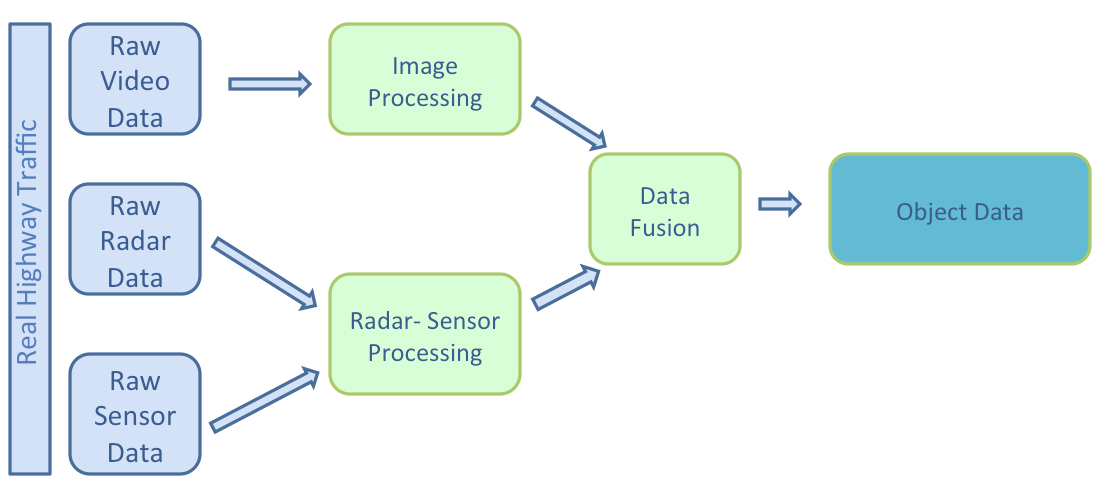
\includegraphics[scale=0.35]{./figures/DaimlerDataFlow}
\caption{\label{Figure:DaimlerDataFlow} Daimler's data flow.}
\end{center}
\end{figure}

Figure \ref{Figure:DaimlerDataFlow} contains a visual description of the current data flow used to create the ``object data''.  First, the raw data coming from the video, radar, and sensors are preprocessed. Then, the preprocessed data is merged, and the high-level or ``object data'' describing the traffic scene is obtained. 

As commented above, using the resulting ``object data'', Daimler has developed a probabilistic graphical model \cite{kasper2012object} which is able to recognize an ongoing manoeuvre around 0.6 seconds before it really takes place.  This probabilistic approach is based on modelling the problem in different abstraction layers. 


%The sensor data is modelled in the first layer. Using this layer, a new layer is created on top with the goal of detecting a lane change behaviour. The detection of a lane change behaviour allows the system to model the lane change manoeuvre in a higher layer. Finally, with this information, the system is able to identify the kind of driving manoeuvre which is taking place between a pair of vehicles. 
%
%
%
%\begin{figure}
%\begin{center}
%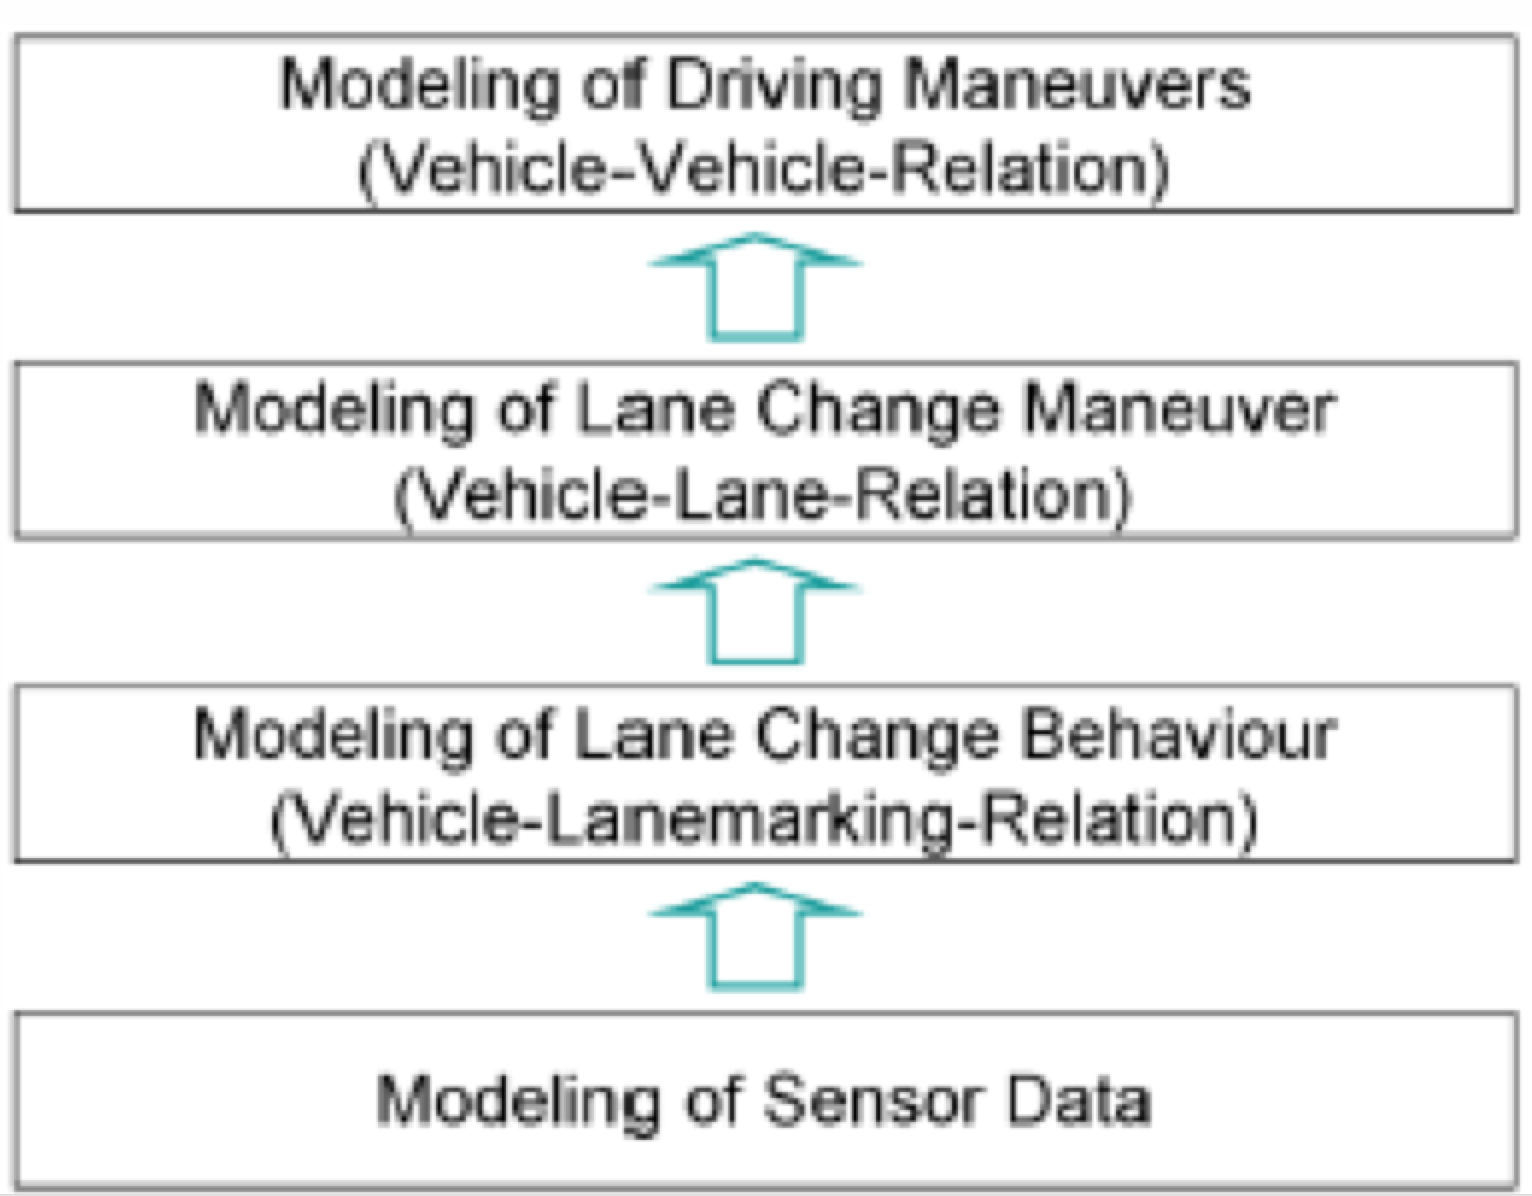
\includegraphics[scale=0.58]{./figures/DaimlerHierarchicalModelling}
%\caption{\label{Figure:DaimlerHierarchicalModelling} Hierarchical layers for the recognition of driving manoeuvres.}
%\end{center}
%\end{figure}

\subsubsection*{Static OOBN model}

The model described here was presented in \cite{kasper2012object} as an object-oriented Bayesian network (OOBN) \cite{KollerPfeffer1997} for addressing the problem of early recognition of a lane change manoeuvre (application scenario 1).  This model works with the so-called ``object data''. This data mainly consists of a set of measured and/or computed signals or situation-features denoted by $S$ (e.g. EGO speed, EGO lateral velocity, speed of a car in-front, etc., see \cite{kasper2012object} for further details) describing the traffic scene. The situation features used for manoeuvre recognition are structured along three main dimensions: lateral evidence (LE), trajectory (TRAJ), and occupancy schedule grid (OCCGRID).  A visual description is given in Figure \ref{Figure:DaimlerSituationFeatures}. They are referred to as the three possible hypotheses of a lane change manoeuvre: 1) LE hypothesis considers the lateral offset and the lateral velocity of a car and accounts for its lateral movement; 2) TRAJ hypothesis accounts for the evidence about a car's trajectory by using the measures of the car angle and the estimated time to crossing the line; and 3) OCCGRID hypothesis allows to identify if a car surroundings are going to be occupied by some other vehicle in the traffic scene. 

\begin{figure}
\begin{center}
\begin{tabular}{ccc}
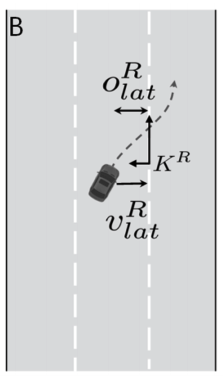
\includegraphics[scale=0.5]{./figures/DaimlerLEHipothesis} &

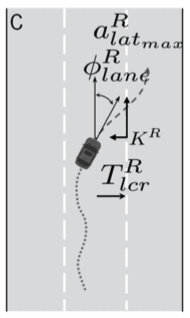
\includegraphics[scale=0.5]{./figures/DaimlerTRAJHipothesis} &

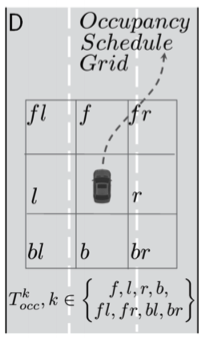
\includegraphics[scale=0.5]{./figures/DaimlerOCCGRIDHipothesis} \\

Lateral evidence & Trajectory & Occupancy grid \\
\end{tabular}
\caption{\label{Figure:DaimlerSituationFeatures} The three main dimensions of the situation features \cite{kasper2012object}.}
\end{center}
\end{figure}

%The whole modelling is structured in hierarchical layers as detailed in Figure \ref{Figure:DaimlerHierarchicalModelling} and it has been previously implemented \cite{kasper2012object} using an object-%oriented Bayesian network (OOBN) \cite{KollerPfeffer1997}. 
%Even using this high-level features, the modelling problem is very complex. 
%At the same time, the problem contain a lot of structure and can be divided in simpler and similar sub-problems. For example, when deciding whether there is evidence or not that a car is performing a %lateral movement to the right, we can employ two situation-features such as the lateral velocity to the right and the lateral offset w.r.t. the right lane marking of this vehicle to make this decision. But %we will find a quite similar problem when deciding about the lateral movement evidence of the EGO car or any other car, when the only difference that will use another situation-features (e.g. the right %lateral velocity of the EGO) .

The general structure of this OOBN model consists of a number of abstraction levels as detailed in Figure \ref{Figure:DaimlerOOBNAbstraction}: 

\begin{description}
\item[Class sensor measurement:]  This class represents objects at the lowest level of the OOBN. It models the so-called \textit{measured data} which are  the observations characterising a situation. They are acquired from sensors and computations (see Figure \ref{Figure:DaimlerDataFlow}). The structure is the common one found in a standard Kalman filter model to account for sensor noise or fault: S\_MEAS refers to the sensor-reading value, S\_REAL refers to the real value, and S\_SIGMA refers to the uncertainty in the measurements. In this way, the sensor-reading of a measured variable (S\_MEAS) is conditionally dependent on random changes in the real value under measurement (S\_REAL) and sensor noise/fault (S\_SIGMA). In Daimler, the observations of the measured value S\_MEAS and the uncertainty of the measurement S\_SIGMA are given in the object data. 

\item[Class hypothesis:] This class pertains to a higher level and directly depends on the real values S\_REAL obtained in the previous class. In fact, the real sensor values are used to evaluate the different possible hypotheses namely LE, TRAJ and OCCGRID. 

\item[Class event:] This class is at the top level of the modelling. It allows to model high-level Hypothesis/Event based on low-level hypotheses ($Hypothesis_1, \ldots, Hypothesis_n$) in a recursive way. This class also includes the event variable representing the possible traffic manoeuvres of the own and neighbour vehicles. 
\end{description}

\begin{figure}
\begin{center}
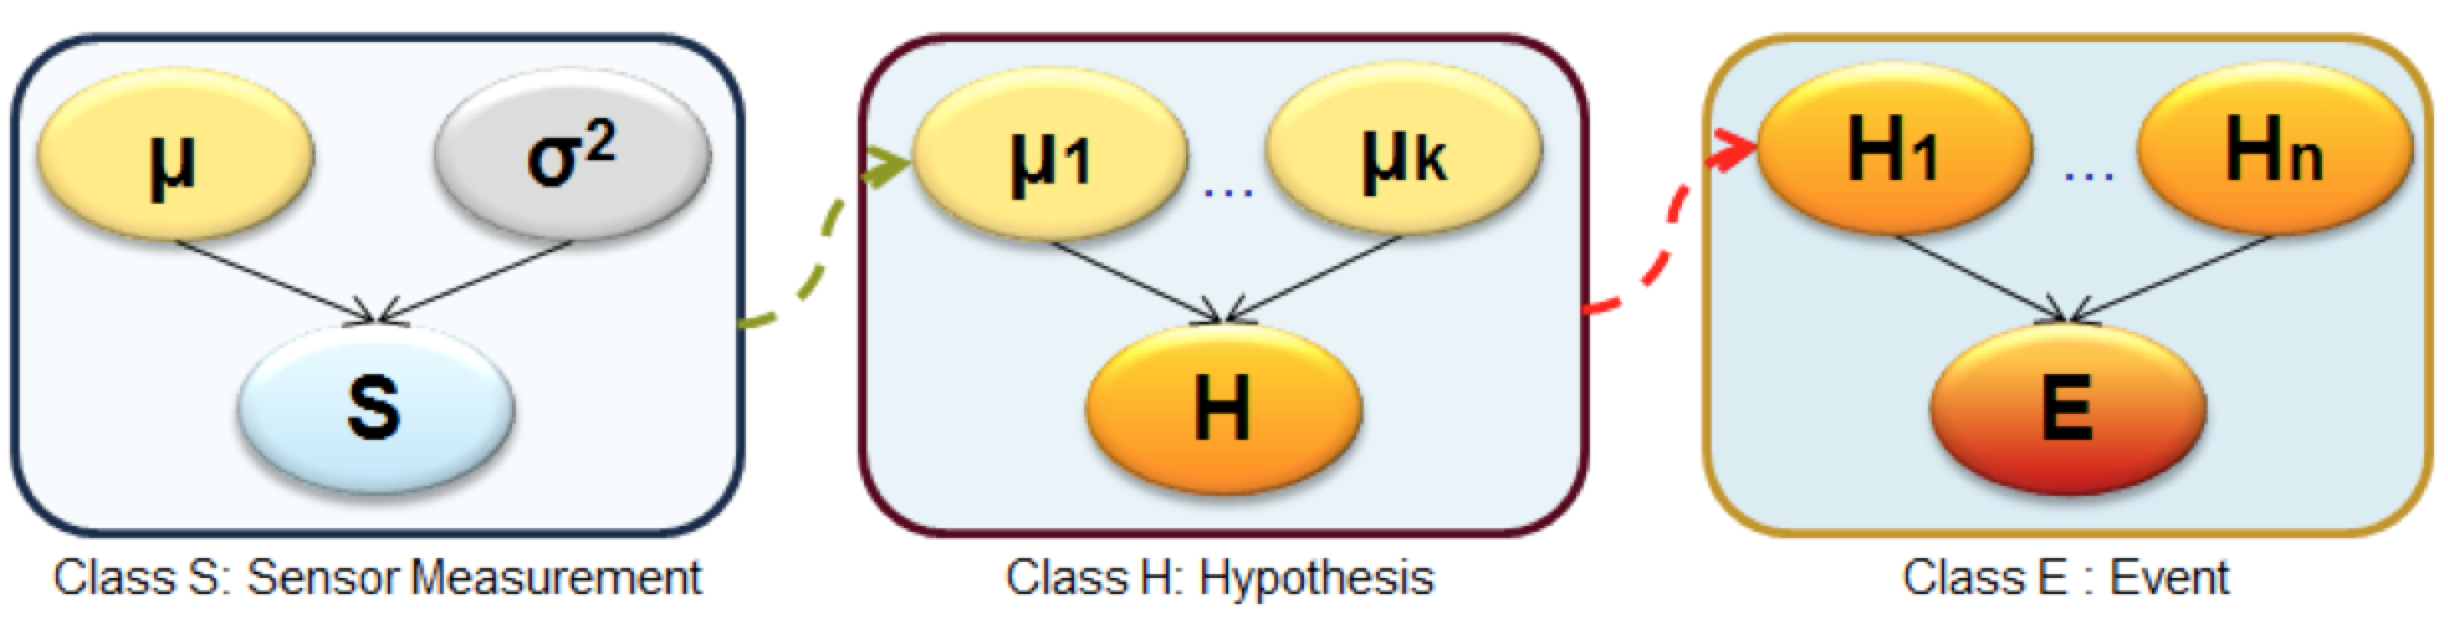
\includegraphics[scale=0.58]{./figures/DaimlerOOBNAbstraction}
\caption{\label{Figure:DaimlerOOBNAbstraction} Static-OOBN model for the prediction of an event (manoeuvre) \cite{Weidl2014}.}
\end{center}
\end{figure}

Finally, Figure \ref{Figure:DaimlerLE} shows a concrete fragment of the static OOBN model related to the LE hypothesis modelling. As it can be seen, LE hypothesis depends on the lateral offset to a lane marking, O\_LAT\_REAL, as well as on the lateral velocity, V\_LAT\_REAL, of the car. Both measures are estimated from their measured values, O\_LAT\_MEAS and V\_LAT\_MEAS, respectively, and from the estimated uncertainty of the measurements,O\_LAT\_SIGMA and V\_LAT\_SIGMA. This OOBN fragment is used to model the growing probability for LE to cross the lane marking, based on the vehicle coming closer to the lane marking and the increase of its lateral velocity.

\begin{figure}
\begin{center}
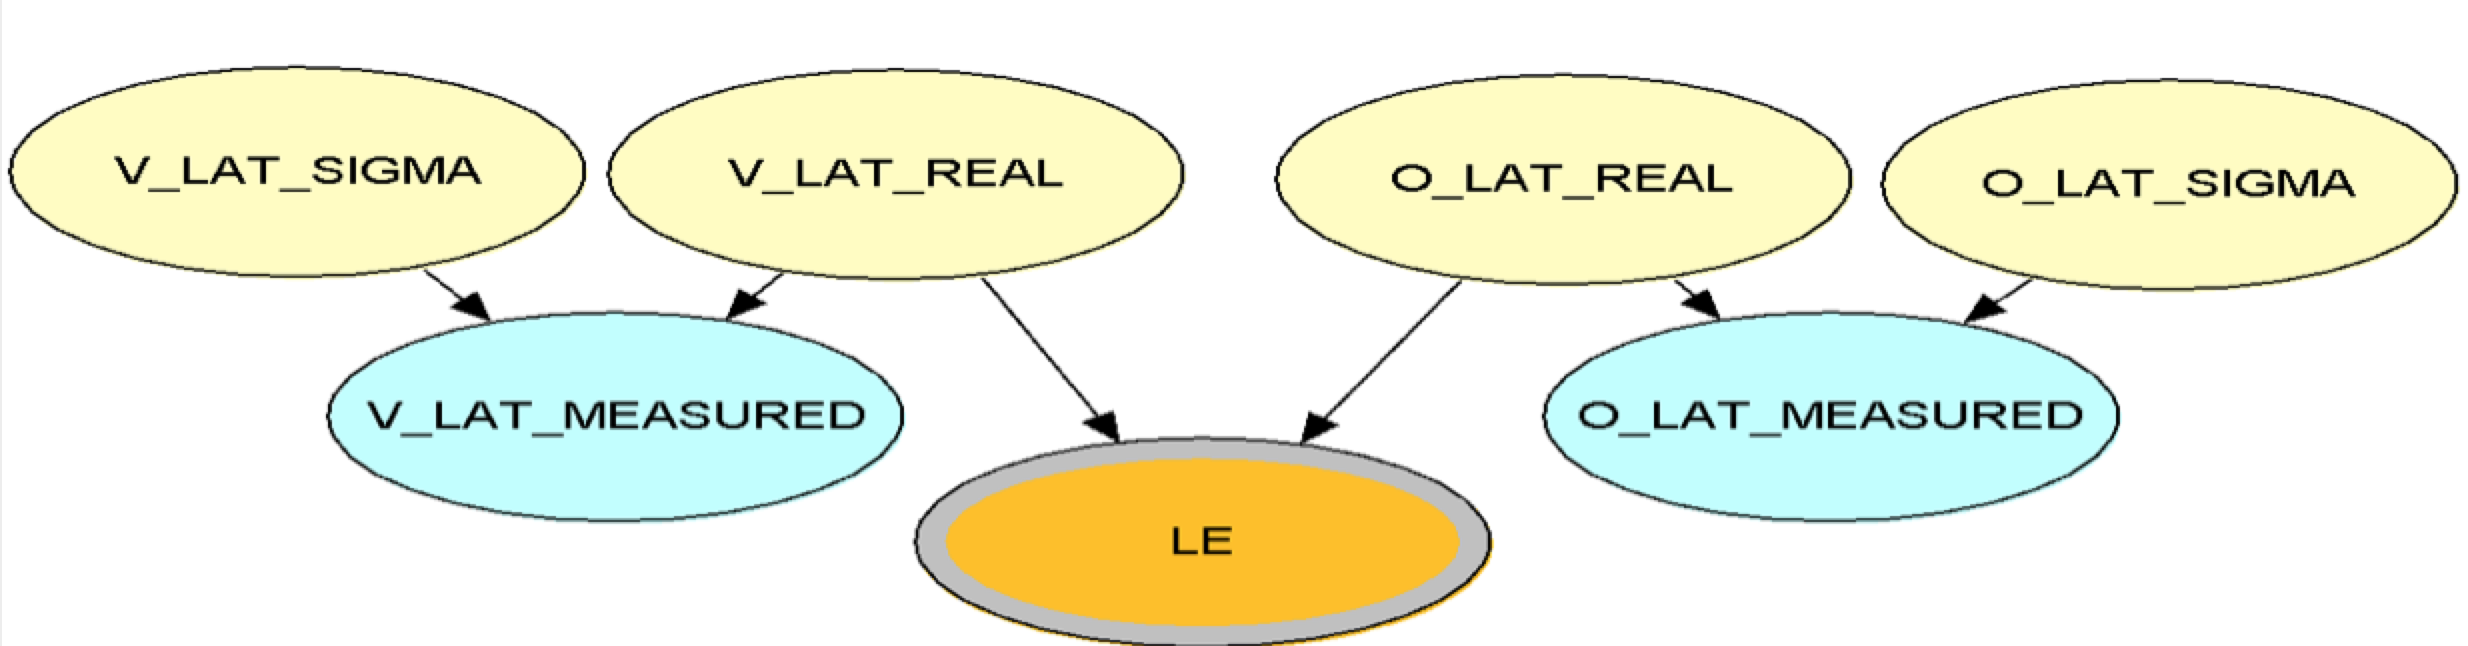
\includegraphics[scale=0.58]{./figures/DaimlerLE}
\caption{\label{Figure:DaimlerLE} Static OOBN fragment for the lateral evidence hypothesis.}
\end{center}
\end{figure}


These models contain both continuous and discrete variables. They were parametrized using the CLG framework \cite{JensenNielsen2007,lauritzen1996graphical} for continuous children with continuous parents and multinomial distributions for discrete children with discrete parents. In these models we also have the case of discrete children with continuous parents (i.e. low-level hypothesis depending of S\_REAL variables) that were initially parametrized by a logistic function. However, as discussed in Section \ref{Section:Preliminaries}, this modelling has significant impact when making inference. A possible solution used in \cite{kasper2012object} is to discretize S\_REAL variables. In this case, because S\_MEAS, S\_SIGMA are always observed their potentials can be collapsed/combined with the potential of the respective discretized S\_REAL variables. And, therefore, all the inferences in this probabilistic model can be made by only using discrete potentials \cite{JensenNielsen2007}.
